\documentclass{article}
\usepackage{amsmath, amssymb}
\usepackage{bm}
\usepackage{graphicx} % Required for inserting images
\usepackage{tikz}
\usepackage{float}
\usepackage[round]{natbib}
\usepackage{hyperref}
\hypersetup{
    colorlinks,
    linkcolor={red!50!black},
    citecolor={blue!80!black},
    urlcolor={red!50!black}
}
\usepackage{setspace}

\usepackage[autostyle]{csquotes}




\bibliographystyle{plainnat}
\usepackage[a4paper, top = 2.5cm,
                     bottom = 2cm,
                     left = 2cm,
                     right = 2.5cm]{geometry}


\title{Private provision of public goods in endogenous renewable resource networks}
\author{Simon Jean}
\date{January 2024}


%%%%%%%%%%%%%%%%%%%%%%
\newcommand*{\xMin}{0}%
\newcommand*{\xMax}{5}%
\newcommand*{\yMin}{0}%
\newcommand*{\yMax}{3}%


\newtheorem{assumption}{Assumption}

\begin{document}
\onehalfspacing
\maketitle
\begin{abstract}
Zebi l'abstract
\\
\textbf{Keywords: } Renewable resources, Ecosystem Health, Dynamic Programming, Network, Graph Theory;
\end{abstract}


\section{Introduction}
% accroche sur la connectivité en économie et les réseaux écologiques

Species productivity and their mobility interact with the evolution of land patterns and determine the distribution and resilience of animal populations. For example, in the Rockies, high annual productivity and dispersal capabilities confer resilience to wolves even in the face of modest human disturbance , while grizzly bears are less resilient, because of their low productivity and dispersal \citep{weaver_resilience_1996}. Moreover, as mean and variances of temperatures, rainfall, wind speed, snow and ice cover are moving with climate change, they could directly and indirectly affect the dispersal of species, through the success of migration and the quality of habitat (see \cite{travis_dispersal_2013}). 
% Les espèces sur les terres : ça fait du bien mais ça coute cher - chasse par exemple

Landowners with valuable resources not only harvest (or cull) the populations on their land, but also increasingly integrate ecosystem health indicators to maintain their long term profit \citep{loreau_biodiversity_2003, baumgartner_economic_2014} . In the case of renewable goods, connectivity has been shown to increase ecosystem resilience \citep{shackelford_role_2018}, and therefore to secure long term profits, as it avoids local extinctions \citep{iucn_iucn_nodate, newbold_global_2014}


 In several locations, landowners have been shown to contribute to ecosystem health along with maximizing their profitability. For example, in the UK, the \href{https://www.nationalgamekeepers.org.uk/articles/deer-initiative-announcement}{Deer Initiative} operated between 1995 and 2020 to \enquote{promote the sutainable management of wild deer}, recognizing that coordination between landowners to manage the population \enquote{on a landscape scale} was paramount to limit the ecological and economic costs of the deer population. This example illustrates how landowners who manage a renewable resource also tend to contribute to a local public good. Not only do they decide on their harvest, they also tend to think about how their land connects to other patches, and to modify their connectivity patterns. 
% Wildfires

In the case of public bads, such as invasive pests, or wildfire risk, landowners tend to minimize the damages they face and also contribute to local public goods. They shape local networks of organization and attempt to shape the distribution of ecological phenomenons. For example, the \href{https://www.nfpa.org/education-and-research/wildfire/firewise-usa}{Firewise Community Program} helps communities design coalitions among different stakeholders such as \enquote{public and private land managers, home owners associations and residents}\footnote{See \url{https://www.fs.usda.gov/features/when-your-community-fire-line}}to collectively reduce wildifre risk, and undertake community scale fuel treatments. In this case, not only do landowners tend to their own parcels, but they also modify the connectivity of land patches. 

% Le thème de l'article
In this article, I study how ecological-economic networks, defined as the spatial distribution of species populations, harvests, migratory flows and connectivity expenditure, result from economic decisions pertaining to harvesting and landscape connectivity. Acknowledging the endogeneity of resource connectivity, how do ecological-economic networks emerge? What are the networks structure that emerge depending on the observed heterogeneity in ecological and economic factors? Depending on the care devoted to public goods by private actors? In identifying the dynamic equilibrium network structural properties of networks, under what conditions can the private provision of public goods yield optimal outcomes? As debates surround the behavior of actors in response to network structures, factoring in that they shape the network may change the conclusions regarding the distribution of efforts and the welfare implications of network structure. This article therefore considers the policy levers that may trigger network formation dynamics to reconcile the private and optimal structures. Can spatially differentiated taxes or subsidies on connectivity related activities help? Should policies be individual, or feature a group component, such as agglomeration payments and bonuses?

To answer these questions, I develop a model of spatial renewable good model, where land owners maximize their intertemporal profit and a measure of ecosystem health which features a public good nature. Landowners have several decision margins. First, they decide how much they harvest the resource. Second, they can improve or degrade inbound and outbound connectivities, depending on how much they fence their land in a given direction, or bait resources from connected patches. In this model, economic and ecological heterogeneity (eg heterogeneous net benefits from harvesting, baiting and fencing, ecological productivities and natural bounds to connectivity) endogenously shape the structure of the network i.e. the connectivity between land patches. I solve the optimality conditions for the dynamic network formation game for a social planner, and for the non-cooperative case. Using a graph theoretic framework, I characterize the emerging equilibria. Using a numerical example, I illustrate the optimal and non cooperative equilibria, and the effect of changes in ecological and economic parameters. Eventually, I investigate how a minimal number of policy instruments can be leveraged to trigger an optimal network formation.

%Literature review
This article builds on two strands of literature, related respectively to the optimal harvest of spatial resources and public good provision in networks.
First, in the literature on spatially connected resources, \cite{brown_metapopulation_1997} study a model of metapopulation with private property and a common pool for barnacles in an optimization framework, but assume uniform connectivity accross space. While it paves the way for further research, this approach \textit{de facto} limits the role played by space. \cite{sanchirico_bioeconomics_1999} develop a more general framework of spatial connectivity in a discrete patchy environment, and analyze the consequences of spatial processes in the Clark model of open access fishery. They include dispersal patterns that can depend on relative densities, following a gravity equation. As they adopt an \enquote{open access} perspective, they do not investigate the optimal harvest rules that take into account endogenous dispersal while paving the way for such an analysis. \cite{costello_optimal_2008} develop a discrete, stochastic model for the optimal harvest of a spatially distributed resource. They investigate the presence of interior and corner solutions (e.g. positive or null harvest), and find an elegant, time and state independent general solution to the optimal harvest problem. They find a constant, patch specific harvest rule to be optimal. Economic and biological heterogeneity across space cause different harvest rates. Eventually, dispersal patterns affect optimal harvests. \cite{costello_optimal_2008} thus derive an optimal solution in a state independent context, that does not acknowledge the endogeneity of dispersal processes. My approach acknowledges the endogenous nature of dispersal processes through different action margins, and shows that accounting for the endogenous nature of dispersal changes optimal harvest, and optimal no-take zones. \cite{fabbri_competition_2022} use fixed, weighted directed graphs to model the dynamics of a spatially distributed population that grows linearly. They find similar results to \cite{costello_optimal_2008} in a graph theoretical framework, and show that designing cost effective reserves in an network can be done using the notion of eigencentrality of a graph.  \cite{costello_private_2017} tackles the private eradication of mobile public bads and connects the optimal resource management resource to the public good literature. They consider the non-cooperative equilibrium when private landowners control a stock of a spatially distributed public bad which causes non linear damages and incurs non linear costs of control. They derive the conditions under which the Markov Perfect Nash Equilibrium results in large or low public bad control provision. Depending on the distribution of marginal damages and costs to eradication, they show that subsets of the landscape emerge where eradication is optimal, while others only control. As dispersal remains exogenous, their model can be interpreted as a generalization of \cite{bramoulle_public_2007}, in a directed, weighted graph setting with non-linear payoffs. In the present article, I use a dispersal matrix that depends on choice variables, although constrained by exogenous, immutable parameters. I study how different action margins affect dispersal, and how the interplay between population stocks and connectivity decisions affect the optimal harvesting strategies.\\
\textbf{results}\\

Indeed, pioneering the literature on public goods in networks, \cite{bramoulle_public_2007} characterize the equilibria emerging from varying undirected, unweighted network structures, in the case of linear payoffs to the public good, and show that networks structure can lead to specialization (e.g. optimal contribution \textit{v.} free-riding), where agents position in the network determine if they contribute or not. In their framework, specialization can lead to welfare benefits, when contributors are linked to many other individuals. Eventually, they show that more links can lead to welfare reduction, as access to the public good increases and reduces individual incentives to contribute. \cite{bramoulle_strategic_2014} extend this framework to relate graph theoretical statistics applied to fixed, non directed graphs and the existence, multiplicity, and stability of static Nash equilibria. Using spectral graph theory and potential games with in linear best reply games, they show that the lowest eigenvalue is the key statistic in the presence of strategic substitutes. It measures the direct effects of agents onto one another : when one increases its contribution, others tend to reduce it, triggering chain reactions. When the lowest eigenvalue is large, effects can take multiple directions and Nash equilibria are multiple. With low mininimal eigenvalue, the effects are dampened, and a unique equilibrium emerges. Considering two action margins, \cite{chen_multiple_2018} extend results from the single action margin in the case of quadratic games with linear best-reply functions, thus paving the way to analyze the interplay of multiple action margins in the dynamic equilibrium of ecological economic networks. \cite{elliott_network_2019} focus on non-rival heterogeneous benefits and show that the Pareto efficient outcome can be characterized using a network of marginal externalities in a public good problem. They show that the Pareto efficient is such that the largest eigenvalue of this network is 1. Finally this article extends \cite{griffith_continuous_2022}, who develops a model of network formation allowing for asymetric, weighted links, when agents maximize their utility, including a public good, with continuous links. \cite{griffith_continuous_2022} shows that Nash equilibria, in a static setting, depend on the returns to scale of \enquote{link surplus} (e.g the surplus from forming links). I extend this approach to the case of spatial natural resources, where harvesting and connectivity decisions have returns that depend on others decisions. 
In this article, I adopt a dynamic perspective, and I use graph theoretical statistics to characterize the optimal network (i.e population, harvesting, dispersal) structure,  and the intertemporal Nash equilibria. Indeed, as landowners are concerned about the long term ecosystem health, they dynamically contribute to a public good when deciding how to harvest and invest in connectivity. I account for heterogeneity in initial economic and ecological conditions to characterize the evolution of networks. Eventually, I find policies to reconcile the optimal and non cooperative equilibria and characterize these policies with graph theoretical statistics e.g. eigenvalues. \\
\textbf{results}
%Contributions and results

In section \ref{sec:model}, I set the economic and ecological parts of the model. I describe how dispersal depends on harvesting, fencing and baiting choices, as well as the payoff function for landowners with ecosystem health concerns. In section III, I characterize the optimal network structure etc. 


\section{Model}
\label{sec:model}
\subsection{Population dynamics and dispersal}

Space is divided into $N$ exclusive properties, which I call \enquote{patches}, or as \enquote{nodes} of the ecological-economic network. Each patch $i \in \{1,...,N\}$ has a \textit{given} carrying capacity, which, for simplicity, is proportional to its size $A_i$.
In each patch, at the beginning of period $t$, the landowner measures inbound and outbound dispersal flows from connected neighbors, then harvest the resource and choses the residual stock (or \enquote{escapement}). 
Denoting $X_{it}$ the population and $h_{it}$ the harvest in patch $i$ and period $t$, the residual stock is $e_{it} \equiv X_{it} - h_{it}$. Based on the observation of passed dispersal flows, it choses how much to fence and bait ($z_{it}^F$ and $z^B_{it}$ )to influence dispersal in the next period $t+1$. Then, the resource grows from the remaining stock depending on patch specific characteristics\footnote{As I focus on a single species, I assume the intrinsic growth rate of the species to be distributed homogenously accross patches}, according to a growth function $g(e_{it}| A_i) \equiv g_i(e_{it})$, with $g_i$ increasing and concave and $g_i(0|A_i)=0$. 

Once the resource has grown, it disperses through space. Dispersal depends on immuable factors such as altitude differential or temperature (eq \ref{eq:dispersal_natural_limits}) and endogenous factors, including relative densities (e.g. between patch $i$ and patch $j$, migration depends on $X_{it}$ and $X_{jt}$) and devices that can increase or reduce inbound or outbound connectivity (eq. \ref{eq:dispersal_dynamics}).
Dispersal from patch $i$ to patch $j$ in period $t$, denoted $d_{ijt}$, depends on relative densities, the amount of fencing and baiting, as well as the immutable factors\footnote{Note that $d_{ijt} \neq d_{jit}$ in general.}, and the observed dispersal in $t$. Figure \ref{fig:dispersal_dyn} shows the evolution of the network between two periods.
Moreover, the sum of outbound migration rates sums to 1 (eq. \ref{eq:dispersal_outbound_flows}): 


\begin{equation}
d_{ij, t+1} \in [\underline{d_{ij}}, \bar{d_{ij}}] \subset [0,1] \label{eq:dispersal_natural_limits}
\end{equation}
\begin{equation}
d_{ij, t+1} = d_{ij, t+1}\left(z_{it}^F, z_{jt}^B, e_{it}/ e_{jt}; d_{ijt}\right) \label{eq:dispersal_dynamics}
\end{equation}
\begin{equation}
\forall i \in \{1,...,\}, \sum_{j=1}^N d_{ijt} = 1
\label{eq:dispersal_outbound_flows}
\end{equation}

Dispersal from patch $i$ to $j$ effectively depends on the relative amount of fencing from $i$, and baiting from $j$. If $i$ fences its land, dispersal (weakly) decreases. If $j$ baits, dispersal (weakly) increases. Dispersal depends on the relative density between patch $i$ and $j$: if density is larger in one patch, dispersal (weakly) decreases. Eventually, dispersal in $t+1$ (weakly) grows with 
Overall, equation \ref{eq:derivatives} summarizes these first order effects : 
\begin{equation}
\begin{aligned}
	\frac{\partial d_{ijt+1}}{\partial z_{it}^F} \leq 0 &\text{ and } \frac{\partial d_{ijt+1}}{\partial z_{jt}^B} \geq 0\\	
	\frac{\partial d_{ijt+1}}{\partial e_{it}	}  \leq 0 & \text{ and }\frac{\partial d_{ijt+1}}{\partial e_{jt}	}  \geq 0 \\
	\frac{\partial d_{ijt+1}}{\partial d_{ijt}} & \geq 0
\end{aligned}
\label{eq:derivatives}
\end{equation}

The timing of the model is illustrated in figure \ref{fig:timing}. Overall, the population stock in patch $i$ at the beginning of period $t+1$ before harvest and dispersal, is the difference between the inbound migration flows and outbound migration flows : 
\begin{equation}
X_{i,t+1} = \sum_{i=1}^N d_{ji,t+1}\left(z_{jt}^F, z_{it}^B, e_{it}, e_{jt}; d_{ijt}\right) g_j(e_{jt})
\label{eq:resource_dynamics}
\end{equation}



The landscape can be viewed as a directed weighted graph $\mathcal{G}_t = (V_t, E_t)$, with nodes (or vertices) $V_t = \{1,..., N\}$, and edges $E_t = \{\forall i,j \in V_t, d_{ijt}\}$. In this case, the adjacency matrix is denoted $\mathbf{D}_t \in \mathbb{R}^{NxN}$, with diagonal elements denoting self-retention, and $\mathbf{D_t}\mathbf{1}_N = \mathbf{1}_N$ with $\mathbf{1}_N$ the $N\times 1$ vector of 1s. Note that $\mathbf{D}_t$ can be decomposed in two matrices, following \cite{fabbri_competition_2022}, where $\mathbf{A}_t$ denotes self retention rates, while $\mathbf{M}_t$ denotes the outbound migration rate:

\begin{equation*}
\mathbf{A}_t\left(\mathbf{z^F}, \mathbf{z^B}, \mathbf{e}_t; \mathbf{D}_t\right) \equiv a_{ijt} = 
\begin{cases}
	&\left(1 - \sum_{j\neq i} d_{ijt}(\cdot...)\right) \text{ if } i=j\\
	&0 \text{ otherwise }
\end{cases}
\end{equation*}

\begin{equation*}
\mathbf{M}_t\left(\mathbf{z^F}, \mathbf{z^B}, \mathbf{e}_t; \mathbf{D}_t\right) \equiv m_{ijt} = 
\begin{cases}
	& d_{ijt}(\cdot...) \text{ if } i\neq j\\
	&0 \text{ otherwise }
\end{cases}
\end{equation*}

Let $\mathbf{g}(\mathbf{e}_t)$ be the $N\times 1$ vector of $g_j(e_{jt})$. The resource dynamics can be rewritten in matrix form as : 
\begin{equation}
\mathbf{X}_{t+1} = (\mathbf{A}_{t+1} \left(\mathbf{z^F}, \mathbf{z^B}, \mathbf{e}_t; \mathbf{D}_t\right)+ \mathbf{M}_{t+1}^T\left(\mathbf{z^F}, \mathbf{z^B}, \mathbf{e}_t; \mathbf{D}_t\right))\mathbf{g}(\mathbf{e}_t)
\end{equation}




\subsection{Management objectives}

\subsubsection{Ecosystem health metrics}
Landowners consciously contribute to landscape ecosystem health. Following \cite{keeley_connectivity_2021}, we consider connectivity metrics in \enquote{shared ecoscapes}
\footnote{In opposition with \enquote{heavily modified ecoscapes} and \enquote{large, wild areas}, see figure 2 in \cite{keeley_connectivity_2021}} and adopt both a structural (e.g a species agnostic approach focusing on the physical arrangement of habitat patches, including the presence or absence of barriers or corridors) and functional (e.g a species specific approach, that confronts structural connectivity with actual ecological processes including dispersal ability) perspective on connectivity in a population network. We aim to evaluate the connectivity of an existing network, as well as the specific contribution of a node to connectivity to understand where connectivity could be improved.

In this set-up, the quantity of habitat for wildlife is fixed : we are not concerned with ecological restoration of degraded habitat \citep{rohr_ecology_2018}, we focus on the extent to which a given habitat is connected. In this sense, we assume that the initial landscape configuration is in equilibrium from a long term dynamic that exhausted land use opportunity costs. I use ecosystem health indicators that focus on the intensity of connectivity \textit{between} habitat patches, with a fixed landscape. Note that this does not preclude heterogeneous patch sizes.

A common goal in conservation is to maximize species richness (eg total population) in the landscape over time, or to minimize the risk of local extinction \citep{nicholson_new_2006}. In order to minimize the probability of local extinction (absent harvesting) in a network, patches have to be connected and form a dense network. For each node $i$ in the ecological network, let the $\underline{\mathcal{D}_{it}}$, the inbound degree of node $i$ in period $t$ be the number of nodes that send migratory flows from $j$ to $i$:

\begin{equation}
\underline{\mathcal{D}_{it}} = \big|\{j \in \{1, ..., N \}, d_{jit}>0\} \big|
\end{equation}

And $\bar{\mathcal{D}_{it}}$ be the outbound degree of node $i$ in period $t$ be the number of nodes that send migratory flows from $i$ to $j$ : 

\begin{equation}
\bar{\mathcal{D}_{it}} = \big|\{j \in \{1, ..., N \}, d_{ijt}>0\} \big|
\end{equation}


%In a given patch $i$ and period $t$, let the inbound weight be : 
%\begin{equation}
%W_{it} = \sum_{j=1}^N d_{jit}
%\end{equation}

We focus on the distribution of dispersal rates $d_{ijt}$, on the inbound degree distribution, and on the outbound degree distribution rather than on the species richness. Focusing on species richness can lead to an extremely concentrated population\footnote{Assume two patches, $1$ and $2$ such that $\forall X, f_1(X|A_1)>f_2(X|1_2)$, then maximizing richness over time implies $d_{11t}=d_{11}=1 \forall t$ and $d_{22t} = d_{22} = 0 \forall t$. If $\exists \tilde{X}$ such that $\forall X<\tilde{X}, f_1(X|A_1)<f_2(X|A_2)$ and $\forall X>\tilde{X}, f_1(X|A_1)>f_2(X|A_2)$, then maximizing species richness leads to concentrated outcomes depending on the population $X$ in period $t$.}. The landowners aim at maximizing the average inbound weight while minimizing its variance, e.g., at homogenizing the population and area weighted migratory flows\footnote{Indeed, with a homogenous initial distribution of population and size, maximizing the average of the distribution of $\mathcal{R}_{it}$ while minimizing its variance results in a complete network with $d_{ijt}=d_{ij}= \frac{1}{N}$ - see Appendix for a demonstration}. Landowners aim at minimizing the outbound distance between patches and the variance of dispersal rates : 

\begin{equation}
H_t(\mathbf{D}_t) = \alpha \left(\mathbb{E}(\underline{\mathcal{D}_{it}}) - \mathbb{V}(d_{ijt}) \right)
\end{equation}
With $\alpha >0$ a weight given to the ecological health objective

\subsubsection{Benefits of harvesting \& costs of connectivity}
In each period, landowners harvest the resource, choose fencing and baiting, and tend to the global ecosystem health. 
First, they earn a net marginal benefit $p_i>0$ from harvesting the resource, 
so that the total benefit is $p_i(X_{it}-e_{it})$/
Second, they choose fencing ($z_{it}^F$) and baiting ($z_{it}^B$) by weighing the future marginal benefits resulting from additional resources to harvest, e.g less outbound migration and more inbound migration, with the  costs of fencing and harvesting, denoted $c_i^F(z_{it}^F)$ and $c_i^B(z_{it}^B)$, such that costs are increasing and convex. 

\subsubsection{Ecological Economic Payoff}
Overall, in each period, a landowner maximizes the following payoff : 

\begin{equation}
\Pi_{it}(e_{it}, z_{it}^F, z_{it}^B) = p_i(X_{it} - e_{it}) - c_{iF}(z_{it}^F)  - c_{iB}(z_{it}^B) + H_t(\mathbf{D}_t)
\end{equation}

\subsubsection{Social planner and uncoordinated equilibria}

\paragraph{The social planner} aims at maximizing the sum of profits over time, taking into account the resource's spatial and temporal dynamics. Formally : 

\begin{equation}
\begin{aligned}
	\max_{\{z_{it}^B, z_{it}^F, e_{it}\}_{t, i \in \{1, ..., N\}}}& \sum_{t=0}^\infty \delta \left(\sum_{i=1}^N \Pi_{it}(e_{it}, z_{it}^F, z_{it}^B)\right)\\
	& \text{subject to eq. \ref{eq:dispersal_natural_limits}, \ref{eq:dispersal_dynamics}, \ref{eq:dispersal_outbound_flows} and \ref{eq:resource_dynamics} and}\\
	& \mathbf{X}_0, \mathbf{D}_0 \text{ given}
\end{aligned}
\end{equation}

\paragraph{The individual patch owner} aims at maximizing its own intertemporal profit : 
\begin{equation}
\begin{aligned}
	\max_{\{z_{it}^B, z_{it}^F, e_{it}\}_{t}}& \sum_{t=0}^\infty \delta \left(\Pi_{it}(e_{it}, z_{it}^F, z_{it}^B)\right)\\
	& \text{subject to eq. \ref{eq:dispersal_natural_limits}, \ref{eq:dispersal_dynamics}, \ref{eq:dispersal_outbound_flows} and \ref{eq:resource_dynamics}}\\
	& \mathbf{X}_0, \mathbf{D}_0 \text{ given}
\end{aligned}
\end{equation}

\section{Results}
\subsection{The optimal ecological economic network}
\subsubsection{An illustrative example}
\textbf{Show the first order conditions etc}
For illustrative purposes, assume a 3 nodes graph and two periods (the world starts in $t=0$ and ends in $T=2$). Consequently, there is no investment realized in $T=2$, and the resource is entirely harvested, in every patch. 

\paragraph{Ecosystem health is absent from decisions}
First, consider a case where landowners maximize their profit absent any concern for ecosystem health ($\alpha = 0$). The social planner solves : 

\begin{align*}
& \max \sum_{i=1}^3 \left(\Pi_{i1} + \delta \Pi_{i2}\right)\\
\iff	 &\max  \sum_{i=1}^3 \left[ p_i (X_{i1}-e_{i1}) - c_{iF}(z_{i1}^F) - c_{iB}(z_{i1}^B) + \delta p_i \left( \sum_{j=1}^3 d_{ji2}(z_{j1}^F, z_{i1}^B, e_{i1},e_{j1}, d_{ij1})g_j(e_j)\right) \right]
\end{align*}

First order conditions for each patch $i$ are : 
\begin{align*}
-p_i + \delta \left[ p_i \sum_{j=1}^3 \left( \frac{\partial d_{ji2}}{\partial e_{i1}}g_j(X_j) \right) + \sum_{i=1}^3 d_{ij2}(\cdot...) \frac{\partial g_i}{\partial e_{i1}}\right] = 0 &\text{ } \forall i\\
- c_{iF}'(z_{i1}^F) + \delta \sum_{j=1}^3 \frac{\partial d_{ij2}}{\partial z_{i1}^F}p_j g_i(e_{i1}) =0  \text{ } &\forall i\\
- c_{iB}'(z_{i1}^B) + \delta  \sum_{j=1}^3 \frac{\partial d_{ji2}}{\partial z_{i1}^B}p_jg_j(e_{j1}) = 0 \text{ } &\forall i\\
\end{align*}
\begin{itemize}
\item Commentary on corner solutions
\item Indeterminacy is lifted from corner solutions
\item May depend on initial conditions
\end{itemize}
\subsubsection{Optimal eigenvalues}

\subsection{Non Cooperative Equilibrium}


%\section{Numerical Illustration}


\section{Conclusion}

\newpage
\section{Appendix}
\subsection{Optimal dispersal with homogenous initial population and patch size}
Let $\forall i, X_{i0}=X$ and $\forall i,j A_i = A_j = A$, to cancel the density-dependent aspect of dispersal flows, and $f(\mathcal{R}_{it})$ be the distribution of $\mathcal{R}_{it}$. 

The objective function is : 
\begin{equation}
\max_{\{ d_{ijt}\}_{i,j \in \{1,..., N\}}} \mathbb{E}(\underline{\mathcal{D}_{it}})  - \mathbb{V}(d_{ijt})
\end{equation}  

Notice that $ \max \mathbb{E}(\underline{\mathcal{D}_{it}}) = N$ and $\min \mathbb{V}(d_{ijt})=0$. Therefore, if $d_{ijt} = d>0$, then $\forall i,j, d_{ijt}^* = \frac{1}{N}$. 


\newpage
\begin{figure}[H]
	\centering
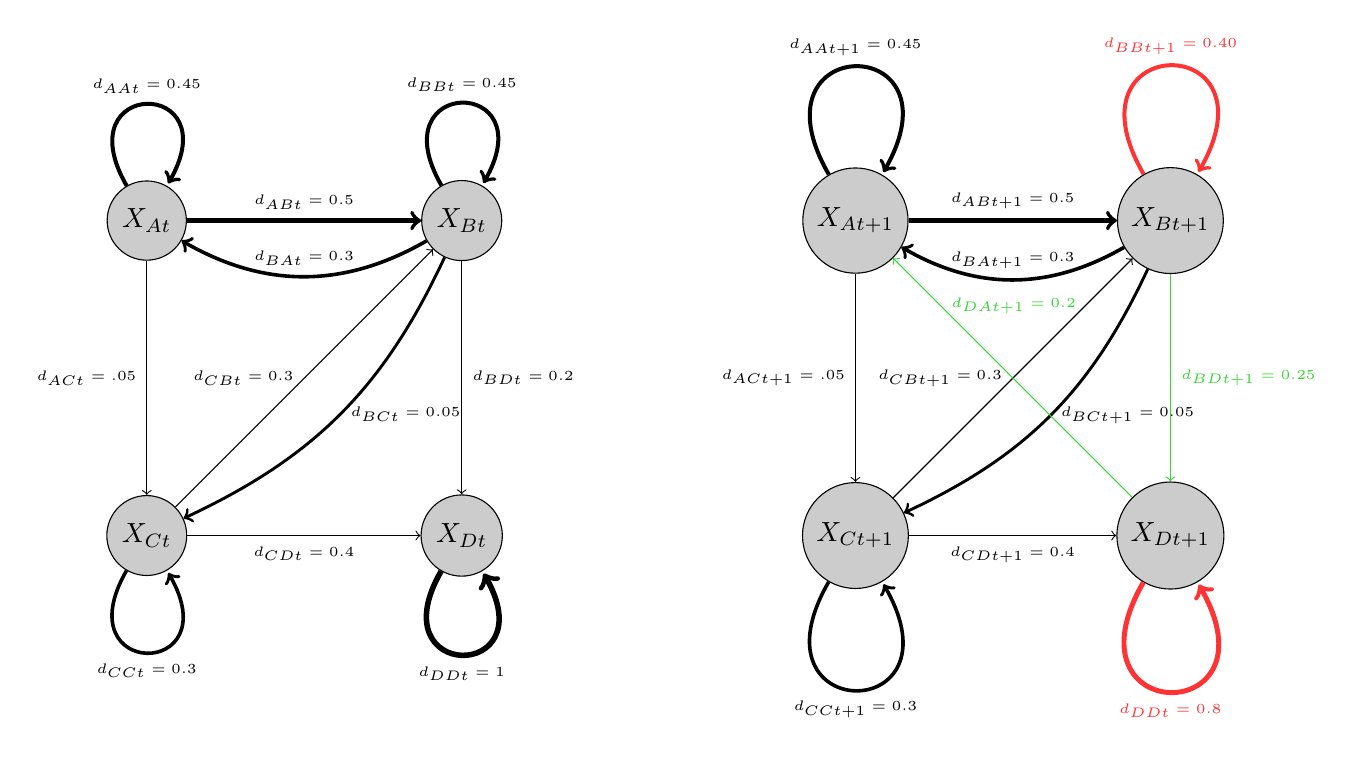
\begin{tikzpicture}

    % Panel 1
     \tikzstyle{circle node} = [circle, draw, fill=black!20, minimum size=1em];

    \begin{scope}[xshift=0cm]
        \node[circle node] (A1) at (0,0) {$X_{At}$};
        \node[circle node] (B1) at (4,0) {$X_{Bt}$};
        \node[circle node] (C1) at (0,-4) {$X_{Ct}$};
        \node[circle node] (D1) at (4,-4) {$X_{Dt}$};
		
		\draw [->, line width = 1.5] (A1) 
			to node[midway,
					anchor = south, 
					font = \tiny] 
				 	{$d_{ABt} = 0.5$} (B1);
        \draw [->, bend left, line width = 1.3] (B1) 
        		to node[midway,  
        				anchor = south,
        			 	font = \tiny] {$d_{BAt} = 0.3$} (A1);

		\draw [->, bend left = 20, line width = 1.05] (B1) 
			to node[midway, 
					anchor = west, 
					font = \tiny] {$d_{BCt} = 0.05$} (C1);
				
        \draw [->] (C1) 
        		to node[midway,  
        				anchor = east, 
        				line width = 1.3, 
        				font = \tiny] {$d_{CBt} = 0.3$} (B1);
        
        \draw [->, black] (A1) 
        		to node[midway, 
        				anchor = east, 
        				line width = 1.05, 
        				font = \tiny]{$d_{ACt} = .05$} (C1);
        				
		\draw [->, black] (C1) 
			to node[midway, 
					anchor = north,
					line width = 1.4, 
					font = \tiny]{$d_{CDt} = 0.4$}(D1);
		
		\draw [->, black] (B1) 
			to node[midway, 
					anchor = west, 
					line width = 1.2,
					 font = \tiny]{$d_{BDt} = 0.2$}(D1);		
		
		\draw [->] (A1) 
			edge [out=120,
				  in=60,loop, 
				  anchor = south, 
				  line width = 1.45, 
				  font = \tiny] node {$d_{AAt} = 0.45$} (A1);
				  
 		\draw [->] (B1) 
 			edge [out=120,
 				  in=60,loop,  
 				  anchor = south, 
 				  line width = 1.45, 
 				  font = \tiny] node {$d_{BBt} = 0.45$} (B1);
 				  
 		\draw [->] (C1) 
 			edge [out=-120,
 				  in=-60,loop, 
 				  anchor = north, 
 				  line width = 1.3 , 
 				  font = \tiny] node {$d_{CCt} = 0.3$} (C1);
 				  
 		\draw [->] (D1) 
 			edge [out=-120,
 				  in=-60,loop,  
 				  anchor = north, 
 				  line width = 2, 
 				  font = \tiny] node {$d_{DDt} = 1$} (D1);
    \end{scope}

    % Panel 2
    \begin{scope}[xshift=9cm]
		\node[circle node] (A2) at (0,0) {$X_{At+1}$};
        \node[circle node] (B2) at (4,0) {$X_{Bt+1}$};
        \node[circle node] (C2) at (0,-4) {$X_{Ct+1}$};
        \node[circle node] (D2) at (4,-4) {$X_{Dt+1}$};
		
		\draw [->, line width = 1.5] (A2) 
			to node[midway,
					anchor = south, 
					font = \tiny] 
				 	{$d_{ABt+1} = 0.5$} (B2);
        \draw [->, bend left, line width = 1.3] (B2) 
        		to node[midway,  
        				anchor = south,
        			 	font = \tiny] {$d_{BAt+1} = 0.3$} (A2);

		\draw [->, bend left = 20, line width = 1.05] (B2) 
			to node[midway, 
					anchor = west, 
					font = \tiny] {$d_{BCt+1} = 0.05$} (C2);
				
        \draw [->] (C2) 
        		to node[midway,  
        				anchor = east, 
        				line width = 1.3, 
        				font = \tiny] {$d_{CBt+1} = 0.3$} (B2);
        
        \draw [->, black] (A2) 
        		to node[midway, 
        				anchor = east, 
        				line width = 1.05, 
        				font = \tiny]{$d_{ACt+1} = .05$} (C2);
        				
		\draw [->, black] (C2) 
			to node[midway, 
					anchor = north,
					line width = 1.4, 
					font = \tiny]{$d_{CDt+1} = 0.4$}(D2);
		
		\draw [->, black, green!80!black!80] (B2) 
			to node[midway, 
					anchor = west, 
					line width = 1.25,
					 font = \tiny]{$d_{BDt+1} = 0.25$}(D2);
					 	
		\draw [->, black, green!80!black!80] (D2) 
			to node[pos = .8,
					anchor = west,  
					line width = 1.2,
					 font = \tiny]{$d_{DAt+1} = 0.2$}(A2);	
		
		\draw [->] (A2) 
			edge [out=120,
				  in=60,loop, 
				  anchor = south, 
				  line width = 1.45, 
				  font = \tiny] node {$d_{AAt+1} = 0.45$} (A2);
				  
 		\draw [->, red!80] (B2) 
 			edge [out=120,
 				  in=60,loop,  
 				  anchor = south, 
 				  line width = 1.45, 
 				  font = \tiny] node {$d_{BBt+1} = 0.40$} (B2);
 				  
 		\draw [->] (C2) 
 			edge [out=-120,
 				  in=-60,loop, 
 				  anchor = north, 
 				  line width = 1.3 , 
 				  font = \tiny] node {$d_{CCt+1} = 0.3$} (C2);
 				  
 		\draw [->, red!80] (D2) 
 			edge [out=-120,
 				  in=-60,loop, 
 				  anchor = north, 
 				  line width = 1.8, 
 				  font = \tiny] node {$d_{DDt} = 0.8$} (D2);
 		
    \end{scope}
\end{tikzpicture}
	\caption{Illustration of dispersal flows within a landscape, and how they evolve between $t$ and $t+1$}
	\label{fig:dispersal_dyn}
\end{figure}


\begin{figure}[H]
  \centering
  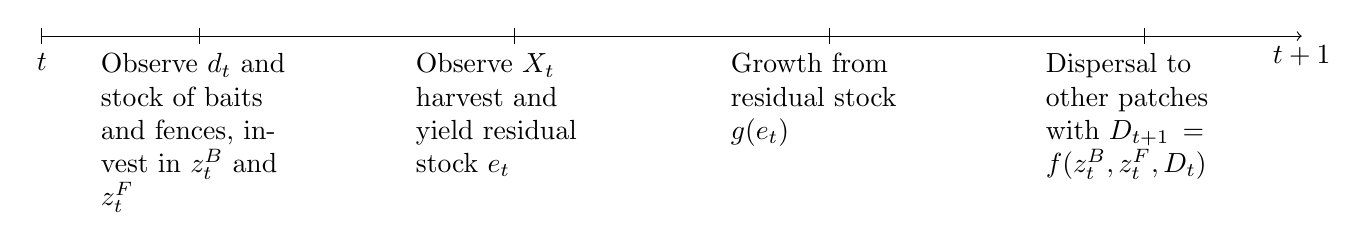
\begin{tikzpicture}
    % Draw the arrow
    \draw[->] (0,0) -- (16,0) node[anchor=north] {$t+1$};
    % Draw ticks and labels
    \draw (0, .1)--(0,-.1) node[anchor = north]{$t$};
    \draw (2, .1)--(2,-.1) node[anchor = north, text width = 2.5cm]{Observe $d_t$ and stock of baits and fences, invest in $z_t^B$ and $z_t^F$};
    \draw (6, .1)--(6,-.1) node[anchor = north, text width = 2.5cm]{Observe $X_t$ harvest and yield residual stock $e_t$};
    \draw (10, .1)--(10,-.1) node[anchor = north, text width = 2.5cm]{Growth from residual stock $g(e_t)$};
    \draw (14,.1)--(14,-.1) node[anchor = north, text width = 2.5cm]{Dispersal to other patches with $D_{t+1}=f(z_t^B, z_t^F, D_t)$};
  \end{tikzpicture}
  \caption{Timing of the model}
  \label{fig:timing}
\end{figure}




\newpage
\bibliography{resources}

\end{document}
